\section{Background}

\todo{complete outline; fill}
\begin{outline}[enumerate]
\1 Overview of LANDIS-II as a process-based landscape model.
\1 Overview of current modeling efforts for soil biota dynamics.
\2 current recognition of the role of soil biota in seral succession and community composition 
\2 limitations and omissions of CENTURY
\1
\end{outline}


\section{Questions}

\todo{complete outline; fill}
\begin{outline}[enumerate]
\1 Is it possible to use the outputs from LANDIS-II simulations to predict soil organic carbon dynamics based on rhizodeposition and soil food web classes rather than solely on decomposition-based (anaerobic) carbon pools?
\1 Is it possible to use the outputs from LANDIS-II simulations to predict successful patterns of agroecological mutualism?
\1
\end{outline}


\section{Hypotheses}

\todo{develop}


\section{Objectives}
The main objective of this chapter is to construct an extension to LANDIS-II for modeling and evaluation of agroecological landscapes. LANDIS-II is an open-source, spatially-explicit, process-based simulation model of LANdscape DIsturbance and succession. Implicit in this objective is the need to develop the theoretical relationships for linking belowground soil food webs to aboveground productivity.
The AgroEV extension should:
\begin{enumerate}
  \item \textit{Evaluate the process of agriculture through the lens of agricultural-ecological patterns and designs in the context of the mechanisms of agroecological mutualism} -- AgroEV must be able to discriminate between agricultural practices (temporal and spatial designs) based on fundamental ecological relationships between belowground soil food webs and aboveground net primary productivity. 
  \item \textit{Define a new algorithm for modeling the linkage between soil biodynamics and ecosystem processes that explicitly accounts for soil food web functionality and biodiversity} -- AgroEV must be able to incorporate concepts and understandings about plant-soil microbe relationships in such a way that while recent advances in rhizospheric biodynamics can be specifically acknowledged, future states of knowledge will not be excluded. That is, the AgroEV algorithm must be designed for updates, readily incorporating new states of empirically-derived knowledge about plant-soil microbe relationships.
\end{enumerate}



\section{Methods}

\subsection{Theoretical Relationships}
The theoretical development of AgroEV will require new inputs and new functionals for LANDIS-II.  Inputs can be direct measures, literature values, or best-estimates. Many of the mapping functions sketched below are speculative at this point. Ideally, the threshold values for AgroEV outputs ($ O_1, O_2, O_3$) can be determined per unique landscape and subsequently used to evaluate regional-scale designs for agroecological mutualisms (sustainable agriculture). A concept sketch of the AgroEV extension is shown in Figure 1 below.\\

%----------------------------------------------
\noindent \textbf{\underline{Current LANDIS-II inputs}}
%------------------------------------------------
\begin{enumerate}
  \item $a_1$ = Cell area (m)
  \item $a_2$ = Stand area (cells)
  \item $a_3$ = Ecoregion area (cells)
  \item $a_4$ = Plant species  (list)
  \item $a_5$ = Plant species life history data (per spp.)
  \item $a_6$ = Basic soil edaphics (per ecoregion)
  \item $a_7$ = Initial cohorts configuration (per cell)
\end{enumerate}

\vspace{5 mm}
\newpage
%-------------------------------------------
\noindent \textbf{\underline{New AgroEV inputs}}
%-------------------------------------------
\begin{enumerate}
  \item $b_1$ = Biomass counts of soil fungi and soil bacteria ($\mu g / g$ per seral stage per stand)\footnote{Initially, the ratio of soil fungi:soil bacteria will be used as a proxy for soil food web functionality. This may need revision to include the ratio of protozoa:nematodes.)} 
  \item $b_2$ = Concentrations of $Na^{+}, \ Ca^{2+}, \ Mg^{2+}$ (meq/mL soil water extract per ecoregion)
  \item $b_3$ = Cation exchange capacity of mineral soil particles (non-organics only) (meq/100g dirt per ecoregion)
  \item $b_4$ = Depth to a compacted soil layer (or bedrock) (m per stand)
\end{enumerate}

\vspace{5 mm}

%------------------------------------------------------------------------------------------------------
\noindent \textbf{\underline{Spatially-explicit time series data currently generated by LANDIS-II}}
%-------------------------------------------------------------------------------------------------------

\begin{enumerate}
  \item $c_1$ = Species and age (cohort per cell per time)
  \item $c_2$ = Net primary productivity (per cell per time)
  \item $c_3$ = Biomass; aboveground (per cell per time)
\end{enumerate}


\vspace{5 mm}

%-------------------------------------------------------------------------------------------------------------------
\noindent \textbf{\underline{New, spatially-explicit time series data to be generated by AgroEV}}\\
%--------------------------------------------------------------------------------------------------------------------

\noindent \textit{F-series (Mappings1)}
\begin{enumerate}
  \item $F_1$ = Volume of root mass (per cell per time) = $f(a_1, a_4, a_5, b_3, b_4, c_1, c_2)$
  \item $F_2$ = Soil adsorption ratio (per stand per time) = $ {\frac {Na^{+}}{\sqrt {{\tfrac {1}{2}}({Ca^{2+}+Mg^{2+}})}}}$ = $f(b_2)$
  \item $F_3$ = Shannon diversity index for R species (per cell per time) = $-\sum _{i=1}^{R}p_{i}\ln p_{i}$ = $ f(c_1)$
  \item $F_4$ = Biomass; belowground (per cell per time) = $ f(c_2, G_4) $ 
\end{enumerate}

\noindent \textit{G-series (Mappings2)}
\begin{enumerate}
  \item $G_1$ = Rhizospheric density (per cell per time) = $f(F_1, adjacent \ cells)$\footnote{Adjacent cells are from the Moore neighborhood (\verb!http://mathworld.wolfram.com/MooreNeighborhood.html!)}   
  \item $G_2$ = Diversity of photosynthetic carbon inputs; root exudates (per cell per time) = $f(F_3)$
  \item $G_3$ = Diversity of photosynthetic carbon inputs; litter (per cell per time) = $f(F_3, adjacent \ cells)$
 \end{enumerate}  
  
\noindent \textit{H-series (Mappings3)}
\begin{enumerate}  
  \item $H_1$ = Soil food web cohort; a joint, conditional probability distribution (per cell per time) = $ Prob \ (Fungi, Bacteria | G_1, G_2, G_3)$
  \item $H_2$ = The maximum probability of the ratio of soil fungi:soil bacteria, X. The random variable, X is determined by first transforming the soil food web cohort distribution into a new probability distribution of soil fungi:soil bacteria ratios.  Five probability bins are then defined and X selects the bin containing the maximum amount of probability. A second random variable, W assigns a Greek letter as,  
 \end{enumerate}

\[ W = \begin{cases} 
      \alpha  & if \ 0\leq x_{MAX} \leq 0.3  \ (Pioneers) \\
      \beta  & if \ 0.3 < x_{MAX} \leq 1 \ (Early \ seral) \\
      \gamma  & if \ 1 < x_{MAX} \leq 5 \ (Young \ forest)\\
      \delta & if \ 5 < x_{MAX} \leq 100  \  (Mature \ forest)\\
      \epsilon & if \ 100 < x_{MAX}  \ (Old \ growth \ forest))
   \end{cases}
\]

\vspace{5 mm}

%------------------------------------------------------------------------------------
\noindent \textbf{\underline{AgroEV Outputs for Evaluation of Sustainable Ag }}\\
%-------------------------------------------------------------------------------------
\begin{enumerate}
  \item $O_1$ = Soil cation exchange capacity (per cell per time) = $f(b_3, G_4)$
  \item $O_2$ = Productivity index (per cell per time) = $ \frac{Total \ biomass \ accumulated \ in \ the \ system}{Net \ primary \ productivity}$ = $ f(c_2, c_3, F_4)$
  \item $O_3$ = Sequence of Greek symbols generated by the discrete random variable, W  (per cell per time).
\end{enumerate}



\begin{figure}
  \begin{center}
    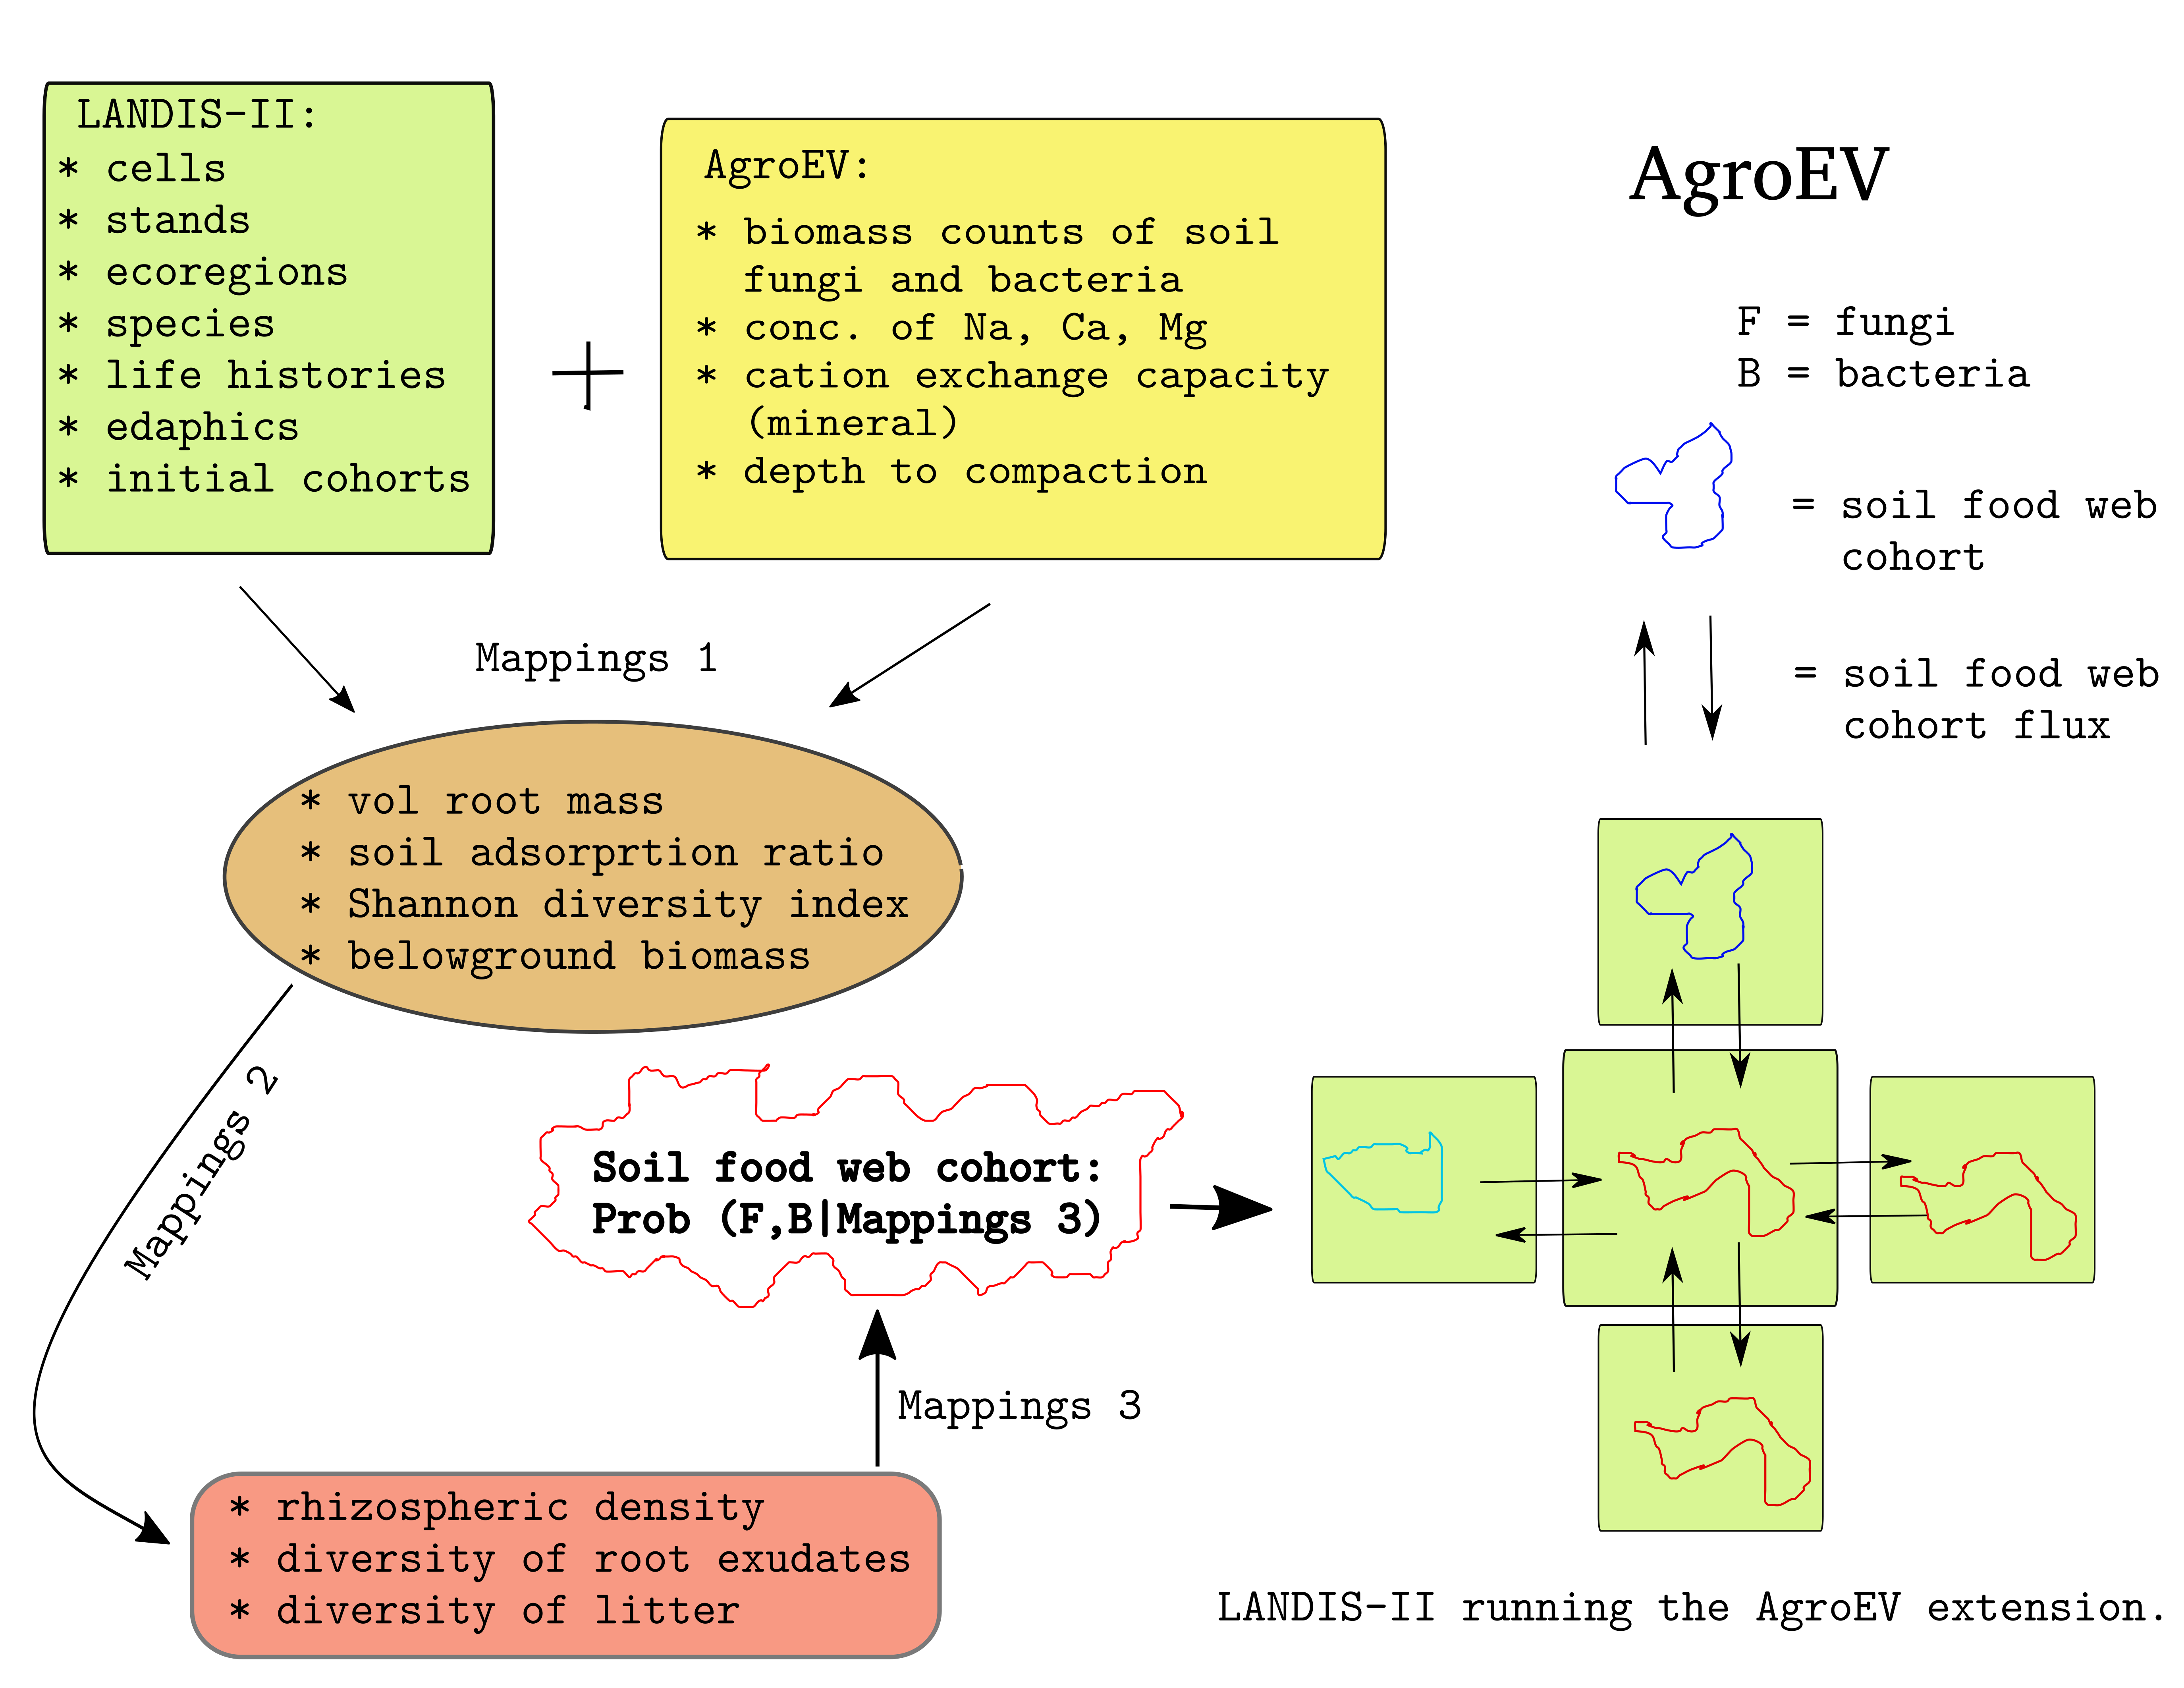
\includegraphics[scale = 0.60]{Ch4_AgroEV/graphics/AgroEV_doc.png}
    \caption{Concept sketch of the AgroEV extension for LANDIS-II.}
    \label{fig:}
  \end{center}
\end{figure}

\newpage
\subsection{Model Construction}
\todo{complete and fill}
\begin{outline}[enumerate]
\1 Use of the LANDIS-II architecture \citep{scheller_design_2007}
\1 Use of standard protocols for simulation model building, verification, and validation \citep{haefner_modeling_2005, law_simulation_2006}
\1 Use of best-practice software engineering plus standard operating procedures for QAQC to produce well-documented C\# code. Best practices and QAQC protocols include the use of GitHub for revision and change control, external code review, unit testing, and work logs. 
\1  
\end{outline}
 
